\section{Experimental Evaluation}\label{sec:exp}

In this part, we first present a case study of the visualizations provided by $\avats$ in Section~\ref{sec:case} to demonstrate its good visualization quality. In Section~\ref{sec:user}, we conduct a comprehensive user study to compare the visualization quality of different methods. In Section~\ref{sec:quality}, we quantitatively evaluate the visual quality and efficiency of $\avats$ and compare with the baselines.

\begin{table}
	\centering
	\small
	\caption{Statistics of the datasets used in the experiments}
	\begin{tabular}{|c|c|c|c|c|} \hline
		Dataset & No. of  & No. of GPS  & Maximum  \\
                & Trajectories & points & length \\ \hline
		\pt{}& 2,389,863 & 75,667,503 & 3,490 \\ \hline
		\sz{}& 3,066,861 & 53,527,890 & 2,268 \\ \hline
		\cd{}& 2,400,000 & 80,040,361 & 6,468 \\ \hline
	\end{tabular}	\label{tab:dataset}
\end{table}

%porto:总条数:2389863,总点数:75667503,最长:3490;  Shenzhen:总条数:3066861,总点数:53527890,最长:2268

\stitle{Experiment Settings} We conduct the experiments
using 3 real-world trajectory datasets: \pt{}, \sz{} and \cd{}.
\pt{}~\cite{pt} contains 2.39 million taxi trajectories and 75.67 million of GPS points, and the longest trajectory has 3,490 GPS points.
\sz{}~\cite{sz} consists of 3.07 million taxi trajectories with 53.53 million GPS points, and the longest trajectory has 2,268 GPS points.
\cd{}~\cite{cd} has 2.40 million taxi trajectories and 80.04 million GPS points, and the longest trajectory consists of 6,468 GPS points. 
The statistics of the datasets are summarized in Table~\ref{tab:dataset}. The experiments are conducted on a machine with an Intel i7-8700 CPU, 24 GB memory and an NVIDIA GeForce GTX1080 GPU with 8 GB on-chip memory, running on Windows 10. All methods are implemented using Java 1.8. UnfoldingMap 0.9.92~\cite{ufmaps} is used to provide interactive map and GPS mapping, and the Processing 3 library~\cite{p3} is used for rendering. All timing results are measured in single-thread mode. The datasets and source codes to reproduce our results are available at~\cite{code}.

\stitle{Competitors} We compare $\avats$ with three competitors, i.e., $\mathsf{Full}$, $\mathsf{Random}$ and $\mathsf{DTW}$. $\mathsf{Full}$ visualizes all trajectories in the user selected region while $\mathsf{Random}$ selects trajectories in the user selected region at random for visualization. $\mathsf{DTW}$ is based on the DTW distance between trajectories~\cite{borcan2012improving} and designed by us to select trajectories with good diversity. Specifically, $\mathsf{DTW}$ samples the trajectory that maximizes the aggregate DTW distance to all remaining trajectories in each step. We note that it takes $\mathsf{DTW}$ several days to run on the experiment datasets because it needs to compute expensive DTW distance (quadratic complexity w.r.t. trajectory length) between all trajectory pairs. For fair comparison, we ensure that $\mathsf{Random}$ and $\mathsf{DTW}$ use the same number of trajectories as $\avats$.




\subsection{Case Study}\label{sec:case}

We conduct case study on the \pt{} dataset to demonstrate the visualization quality of $\avats$. Similar phenomenons are also observed on the other datasets and we omit their results for conciseness.

\begin{figure*}[t]
	\centering
	\includegraphics[width=1\textwidth]{pictures/case_study_icde/case_study_detail.pdf}
	\trim
	\caption{Case study of the visualization quality of $\avats$ for two detail regions.}
	\label{fig:detailview}
	\trim \trim
\end{figure*}

\subsubsection{Overview visualization}

We illustrate the visualization results of different methods for the entire \pt{} dataset in Figure~\ref{fig:overview}.

\stitle{Good visual quality for overview}
At zoom level 11, Figure~\ref{fig:overview}(A) is the visualization result of $\mathsf{Full}$ on the \pt{} dataset.
With a sampling rate $\alpha \!=\! 1\%$, Figures~\ref{fig:overview}(B), (C) and (E) are the visualizations produced by $\mathsf{Random}$, $\mathsf{DTW}$,
and $\avats$, respectively. Comparing with Figure~\ref{fig:overview}(B) and (C), it is obvious that Figure~\ref{fig:overview}(E) is more similar to Figure~\ref{fig:overview}(A). In particular, Figure~\ref{fig:overview}(E) not only preserves the overall visual structure of the entire region but also keeps the details of cities that are far from the center (marked by the dashed cycles in the figure). However, the details of these cities are lost in Figure~\ref{fig:overview}(B) as $\mathsf{Random}$ is more likely to select trajectories in the dense region. $\mathsf{DTW}$ in Figure~\ref{fig:overview}(C) preserves more details than $\mathsf{Random}$ in the sparse regions as it considers diversity in trajectories but its visualization quality is still inferior compared with $\avats$ in Figure~\ref{fig:overview}(E).

\stitle{Good visual quality under different sampling rates}
Figure~\ref{fig:overview}(D) and (E) are the visualizations produced by $\avats{}$ with a sampling rate of $0.1\%$ and $1\%$, respectively. We can make two observations: (i) the larger the sampling rate, the better the visual quality, i.e., Figures~\ref{fig:overview}(E) is more similar to Figure~\ref{fig:overview}(A) compared with Figure~\ref{fig:overview} (D); (ii) the visualization of $\avats$ with a sampling rate of $0.1\%$ (i.e., Figure~\ref{fig:overview}(D)) looks more appealing than the visualizations of $\mathsf{Random}$ and $\mathsf{DTW}$ with a sampling rate of $1\%$ (i.e., Figure~\ref{fig:overview}(B) and (C)) as Figure~\ref{fig:overview}(D) better preserves the visual structures of Figure~\ref{fig:overview}(A).



\stitle{Color encoding effectively mitigates visual clutter} At zoom level 11 and with a sampling rate of $1\%$, Figures~\ref{fig:overview}(E) and (F) are the visualizations produced our $\avats$ and $\cavats$ (i.e., $\avats$ with color encoding), respectively.
Visual clutter is severe for $\mathsf{Full}$ (i.e., Figure~\ref{fig:overview}(A)) and $\avats$ (i.e., Figure~\ref{fig:overview}(E)) because many pixels are visualized for the dense region in the center, which makes it difficult to identify the main routes. The visualization of $\cavats$ in Figure~\ref{fig:overview}(F) alleviates this problem by encoding more representative trajectories with warmer color, making it easier to identify some prominent routes than Figure~\ref{fig:overview}(A) and (E).

\vspace{1mm}
\subsubsection{Detail visualization}\label{sec:detail}




We analyze the visualizations produced by different methods for small areas with details by investigating two regions of interest in the \pt{} dataset in Figure~\ref{fig:detailview}.

%We next present the effectiveness of our proposals with detail views by investigating two regions of interest in \pt{}, the dense region B and the sparse region C(shown as in Figure~\ref{fig:detailview}(8)).

%$\mathsf{Full}$
%$\mathsf{DTW}$
%$\mathsf{Random}$



\stitle{Reduce visual clutter and preserve micro structures for dense region} At zoom level 15, region B in Figure~\ref{fig:detailview}(A) is the center of Porto and has the highest concentration of trajectories. Therefore, $\mathsf{Full}$ suffers from severe visual clutter and it is difficult to identify the road networks in Figure~\ref{fig:detailview}(B1).  $\mathsf{Random}$ and $\mathsf{DTW}$ in Figure~\ref{fig:detailview}(B2) and (B3) reduce the visual clutter to some extent by sampling some trajectories. $\avats$ in Figure~\ref{fig:detailview}(B4) is more successful in reducing the visual clutter of $\mathsf{Full}$ and allows to identify a much larger number of routes. In addition, $\avats$ preserves more micro structures of the trajectories than $\mathsf{Random}$ and $\mathsf{DTW}$, e.g., the circular route in the dashed circular region.

% and causes serious visual clutter, as visualized in Figure~\ref{fig:detailview}(B1).
%For example, the circular structures of the main route(shown as the dashed circular region in Figure~\ref{fig:detailview}(B1)) is unclear.
%$\localavats$ alleviates the visual clutter by preserve the $1\%$ trajectories of the total regions but the clutter is still serious. Furthermore, $\avats$ performs better than $\localavats$ by preserving less trajectories and reduce the visual clutter.


\stitle{Preserve overall layout for sparse region}
At zoom level 14, region C in Figure~\ref{fig:detailview}(A) contains the city of Casino Espinho and has fewer trajectories than the dense region in the center. In this case, the sampling methods need to keep the overall layout of the trajectories  to provide good visualization quality. Compared with $\mathsf{Full}$ in Figure~\ref{fig:detailview}(C1), $\mathsf{Random}$ and $\mathsf{DTW}$ in Figure~\ref{fig:detailview}(C2) and (C3) fail to meet this requirement as they do not show any trajectory for areas far from the city, e.g., in the dashed circle. This makes their entire visualization layout very different from $\mathsf{Full}$. In contrast, $\avats$ in Figure~\ref{fig:detailview}(C4) preserves the trajectories in areas far from the city and has a overall layout similar to $\mathsf{Full}$.

%Region C includes the city of Casino Espinho at zoom level 14, which contains less trajectories than the center of Porto as the visualization result of full dataset shown in Figure~\ref{fig:detailview}(C1).
%Given fix sampling rate $\alpha=1\%$, Figure~\ref{fig:detailview}(C2) indicates the visualization of $\localavats$. This visualization result misses a lot if detail information in this region, because the fix sampling rate preserves too few trajectories which is difficult to guarantee the visual quality.
%While $\avats$ in Figure~\ref{fig:detailview}(C3) performs much better than $\localavats$ as the sampling rate is automatically adjusted to according to the visual quality. In this visualization, the trajectory sketch of Casino Espinho is almost the same as it in Figure~\ref{fig:detailview}(C1), the visualized result of full dataset.

To sum up, the case study shows that $\avats$ effectively mitigates visual clutter with sampling and color encoding. With the quality-aware $\vatss$ sampling algorithm, $\avats$ also provides better visualization quality than $\mathsf{Random}$ and $\mathsf{DTW}$ by preserving the micro structures and overall layout of full visualization.

\subsection{User Study}\label{sec:user}

\begin{figure*}
     \centering
     \begin{tabular}{ccc}
		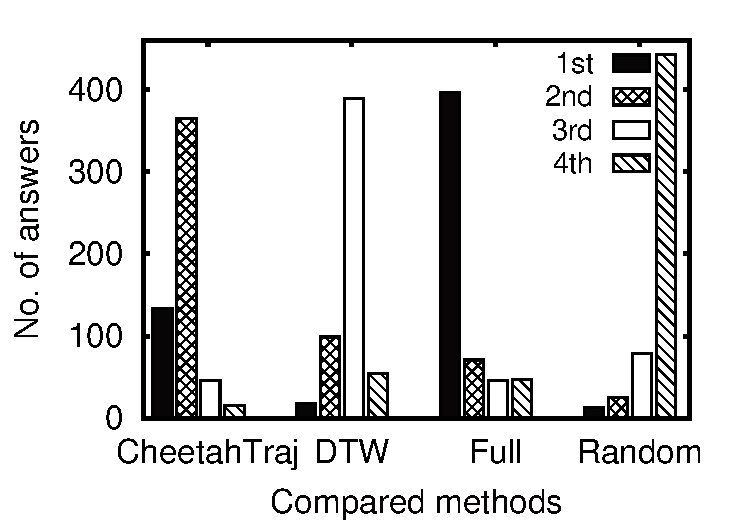
\includegraphics[width=0.6\columnwidth]{pictures/user_study/quality}
		&
		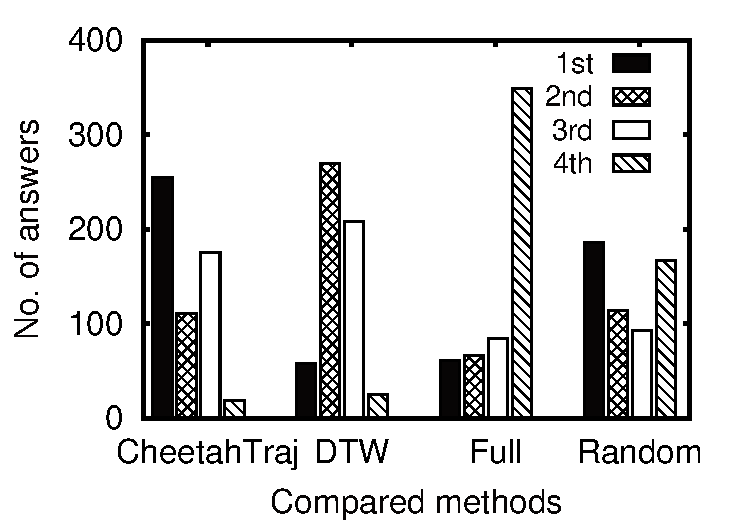
\includegraphics[width=0.6\columnwidth]{pictures/user_study/clutter}
        &
        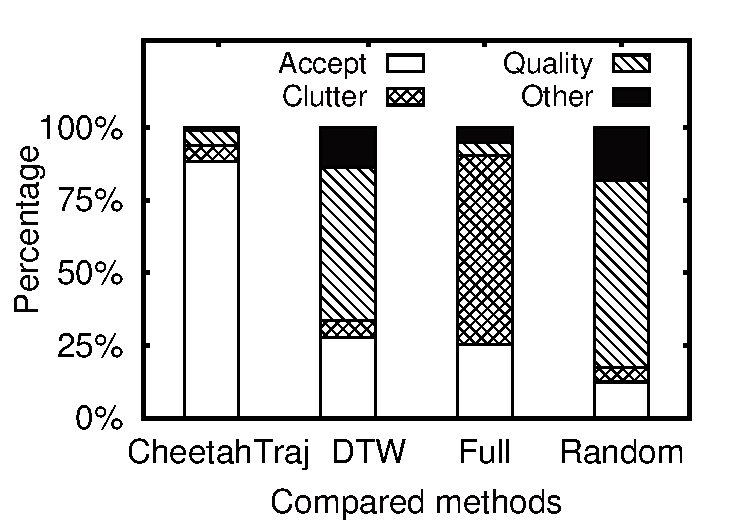
\includegraphics[width=0.6\columnwidth]{pictures/user_study/accept}
		\\
		(A) T1: visual quality study
		&
		(B) T2: visual clutter study
        &
        (C) T3: acceptable visualization study
	\end{tabular}
	\caption{User study results of different visualization methods}
	\label{fig:userstudy}
    \trim
\end{figure*}

In this part, we conduct a user study to evaluate the quality of visualizations generated by different methods objectively.

\stitle{Settings}
We recruited 35 participants with 10 females, 25 males, aged 19 to 31 with a mean of 24.78 for the user study. 
The user study is conducted on the \pt{} and \sz{} datasets, and four visualization methods are investigated, i.e., $\full$, $\rand$, $\mathsf{DTW}$ and $\avats$. We manually select 22 \textit{center points} in the two datasets and define 3 \textit{visualization scales} including:
large-scale region (with zoom level smaller than 13), middle-scale region (with zoom level between 13 and 15), small-scale region (with zoom level larger than 15). For each center point and at each visualization scale, we generate a \textit{comparable visualization group}, which includes one visualization generated by each of the 4 methods. This results in 66 comparable groups (22 center points $\times$ 3 scales) and 264 visualization results (66 comparable groups $\times$ 4 visualizations).

We are interested in the visual quality and visual clutter of the visualizations, and hence designed three tasks for a comparable group:
\begin{itemize}
	\item Task 1 (T1): rank the visualizations in a group from the highest visual quality to the lowest visual quality by 1st, 2nd, 3rd, and 4th.
	\item Task 2 (T2): rank the visualizations in a group from the least visual clutter to the most severe visual clutter by 1st, 2nd, 3rd, and 4th.
	\item Task 3 (T3): select the visualizations considered acceptable (multiple choices allowed) and choose the reason for the visualizations considered unacceptable. We provide three reasons including ``severe visual clutter", ``poor visual quality" and ``others".
\end{itemize}

The user study system is a web-based platform, in which all visualizations are displayed with a resolution of 450*300.


\stitle{User study procedure} When the participants enter the user study system, they are given a tutorial on how to conduct the tasks to get familiar with the interface and tasks.
For each participant, we randomly select 16 comparable groups.
Thus, we obtain $35 \times 16 = 560$ results for each task.
For each comparable group, the 4 visualizations (\textit{without specifying generated by which method}) in it are displayed on the same web-page and a participant is required to perform task T1, T2 and T3 by inspecting them.

%At last, the participants are interviewed to collect feedback after finishing the study and their answers are saved for result analysis.



\stitle{Result analysis} Figure~\ref{fig:userstudy}(A) reports the visual quality ranking of the 4 methods in T1. 
The results show that $\full$ ranks the 1st in most cases while $\avats$ usually ranks 1st or 2nd, i.e., the percentage of $\avats$ ranks top-2 among 4 methods is $88.9\%$. 
In contrast, $\mathsf{DTW}$ and $\rand$ rank 3rd and 4th at most times. 
This suggests that the visualizations generated by $\avats$ are more appealing to the participants than $\mathsf{DTW}$ and $\rand$. 
We also observed that the participants tend to rank $\avats$ before $\full$ for large-scale regions with  many trajectories, and the other way for smaller regions. 


Figure~\ref{fig:userstudy}(B) reports the anti-visual clutter ranking of the 4 methods in T2. 
The results show that visual clutter is most severe for $\full$, ranking 4th in most cases (349 over 560). With sampling, $\mathsf{DTW}$ usually rank 2nd and 3rd but $\rand$ ranks 4th for a considerable number of times as it tends to create clutter in the dense regions.    
$\avats$ is the most successful in reducing visual clutter, ranking 1st in 255 out of the 560 cases and ranking 4th for only 19 cases.    



We report the frequency each of the 4 methods is selected as acceptable and why a method is not selected in T3 using bar chart in Figure~\ref{fig:userstudy}(C). 
Each column corresponds to a method, and from bottom to top, the lengths of the bars indicate the percentage of participants choosing ``acceptable'', ``not acceptable due to visual clutter'', ``not acceptable due to poor visual quality'' and ``not acceptable for other reasons''. 
The results show that $\avats$ is regarded acceptable for about 88.2\% of the cases, and the other methods have significantly lower acceptance rate than $\avats$. 
Specifically, $\mathsf{DTW}$ and $\rand$ have low acceptance rate mainly due to poor visual quality while $\full$ suffers from severe visual clutter.


%Figure~\ref{fig:rank} left shows the ranking among different methods with x-axis indicating the ranking from the highest quality to the lowest quality and y-axis indicating the selecting number for the specific method and ranking. The visualization of $\full$ has the highest visual quality since it has no information loss according the quality definition. The selection of $\avats$ is mostly concentrated at the first and second, which is closely behind the $\full$. The selections of $\baseline$ and $\rand$ are contracted at the third and fourth respectively, which is confirmed both of these two methods performs worse than $\full$ and $\qtavats$ in guarantee the visual quality.



%Figure~\ref{fig:rank} right reports the ranking among different methods with x-axis indicating the ranking from the least clutter to the most clutter and y-axis indicating the total selecting number for the specific method and ranking. We observe that the $\qtavats$ is ranked at the first 155 times which is significantly more than the other methods. The number it ranks at the second, third and last are 68, 96 and 14. There is no doubt that the visualization of $full$ suffers the most sever visual clutter problem because 210 of 333 total answers rank $full$ at the fourth, while other methods can be used to help to reduce the visual clutter.



%\begin{figure}[t]
%	\centering
%	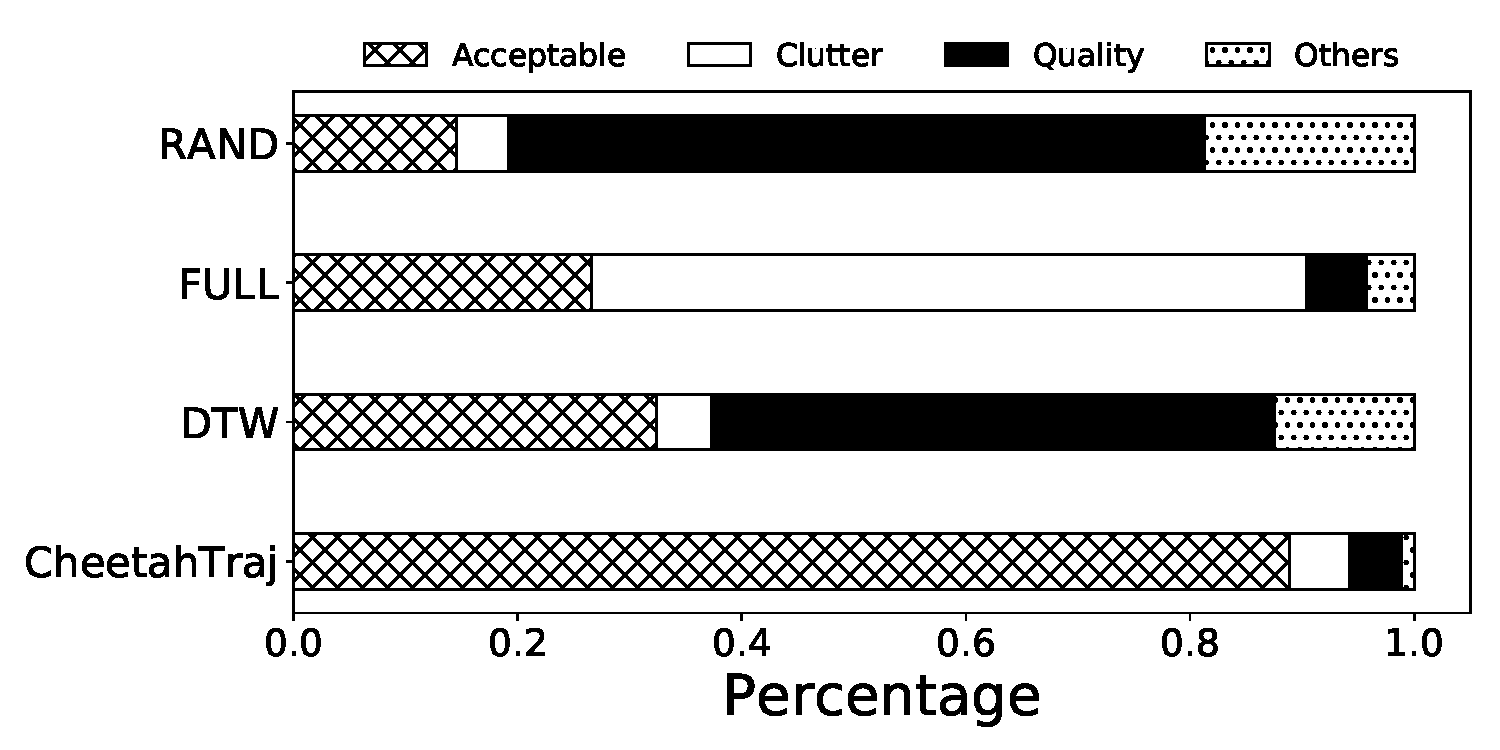
\includegraphics[width=0.35\textwidth]{pictures/user_study/accept_rate.pdf}
%	%\vspace{-5mm}
%	\caption{User study, accept rate.}
%	\label{fig:accept_rate}
%	%\vspace{-8mm}
%\end{figure}






\begin{figure*}
	\centering
	\small
	\begin{tabular}{ccc}
		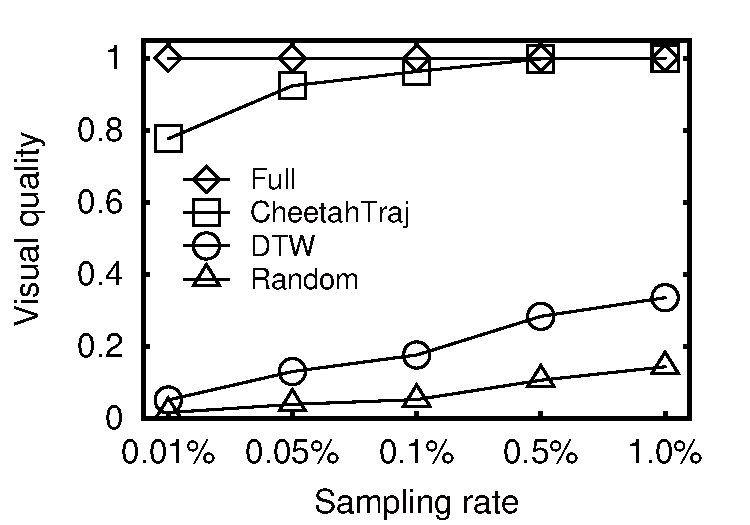
\includegraphics[width=0.3\linewidth]{pictures/quantitative_study/rate_porto_q}
		&
		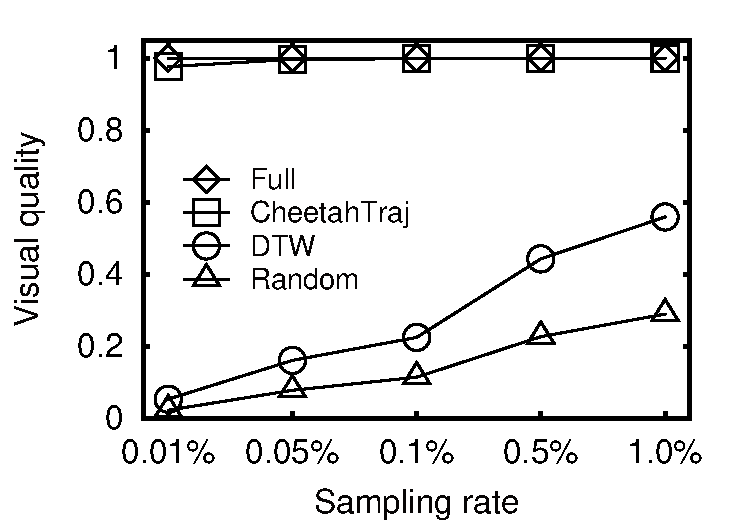
\includegraphics[width=0.3\linewidth]{pictures/quantitative_study/rate_sz_q}
        &
		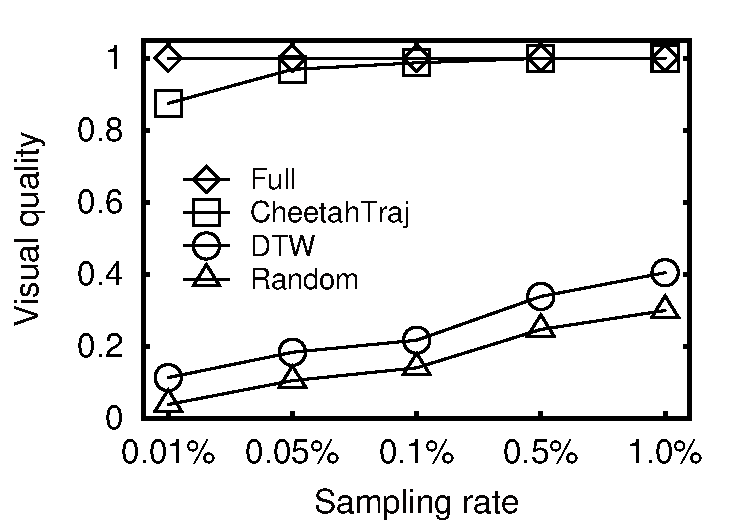
\includegraphics[width=0.3\linewidth]{pictures/quantitative_study/rate_cd_q}
		\\
		(A) \pt{}
		&
		(B) \sz{}
		&
		(C) \cd{}
	\end{tabular}
    \trim
	\caption{Effect of varying sampling rate visual quality.}
	\label{fig:rate_quality}
	\trim \trim
\end{figure*}

\begin{figure*}
	\centering
	\small
	\begin{tabular}{ccc}
		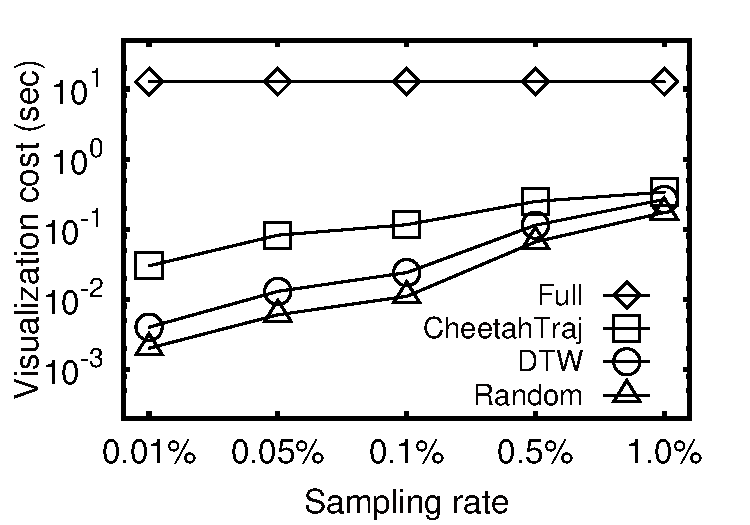
\includegraphics[width=0.3\linewidth]{pictures/quantitative_study/rate_porto_t}
		&
		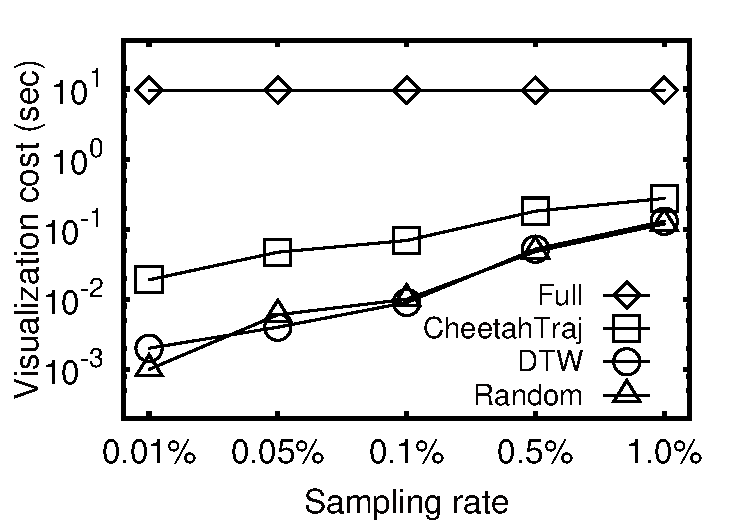
\includegraphics[width=0.3\linewidth]{pictures/quantitative_study/rate_sz_t}
        &
		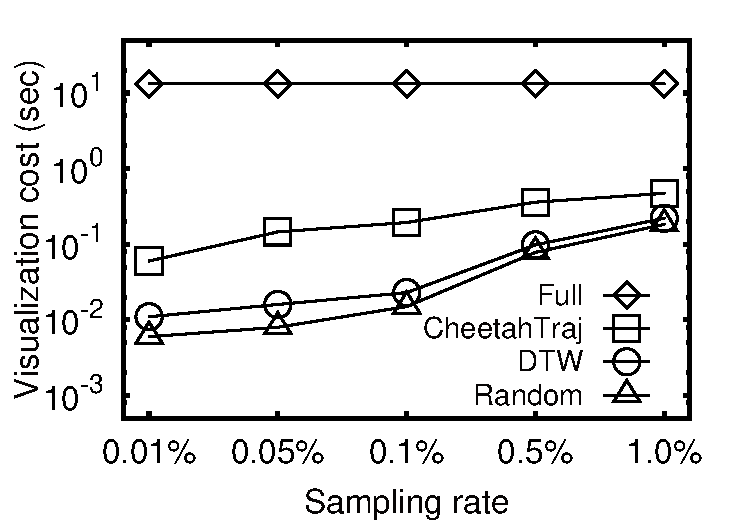
\includegraphics[width=0.3\linewidth]{pictures/quantitative_study/rate_cd_t}
		\\
		(A) \pt{}
		&
		(B) \sz{}
		&
		(C) \cd{}
	\end{tabular}
    \trim
	\caption{Effect of  sampling rate on visualization cost.}
	\label{fig:rate_vistime}
	\trim \trim
\end{figure*}

\begin{figure*}
	\centering
	\small
	\begin{tabular}{ccc}
		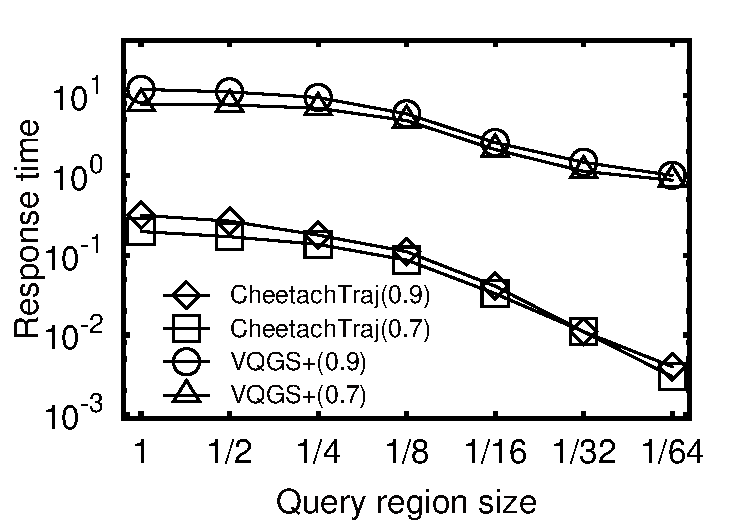
\includegraphics[width=0.3\linewidth]{pictures/quantitative_study/size_porto_t}
		&
		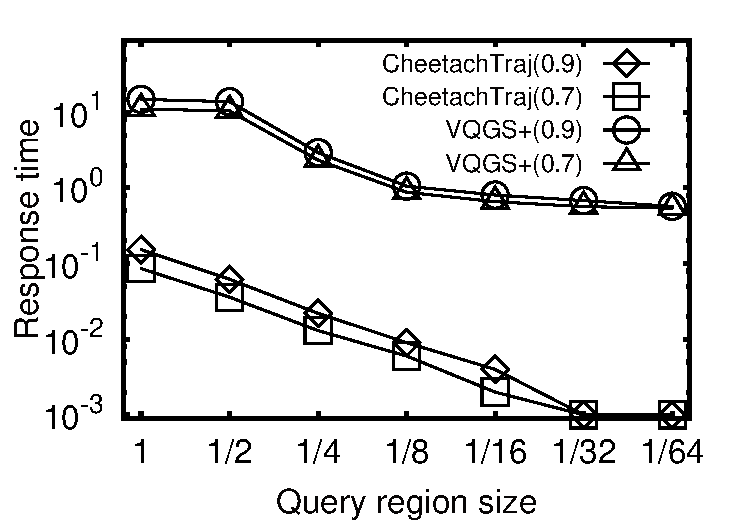
\includegraphics[width=0.3\linewidth]{pictures/quantitative_study/size_sz_t}
		&
		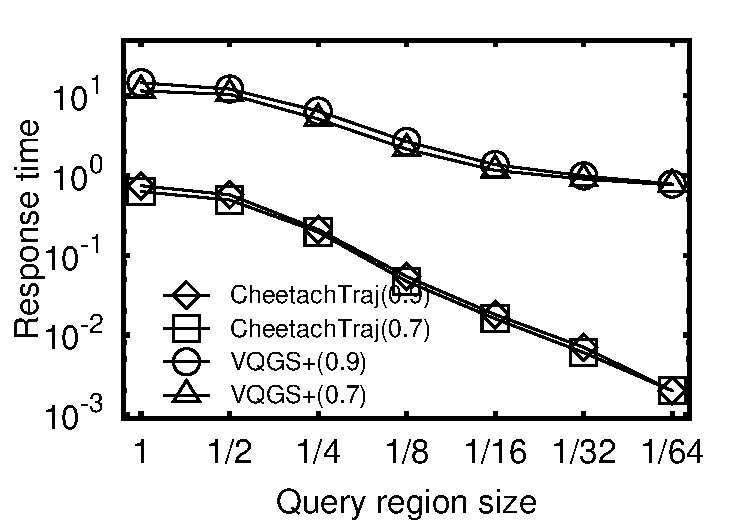
\includegraphics[width=0.3\linewidth]{pictures/quantitative_study/size_cd_t}
		\\
		(A) \pt{}
		&
		(B) \sz{}
		&
		(C) \cd{}
	\end{tabular}
    \trim
	\caption{Effect of region size on end-top-end response time.}
	\label{fig:size_responsetime}
	\trim \trim
\end{figure*}


\begin{figure*}
	\centering
	\small
	\begin{tabular}{ccc}
		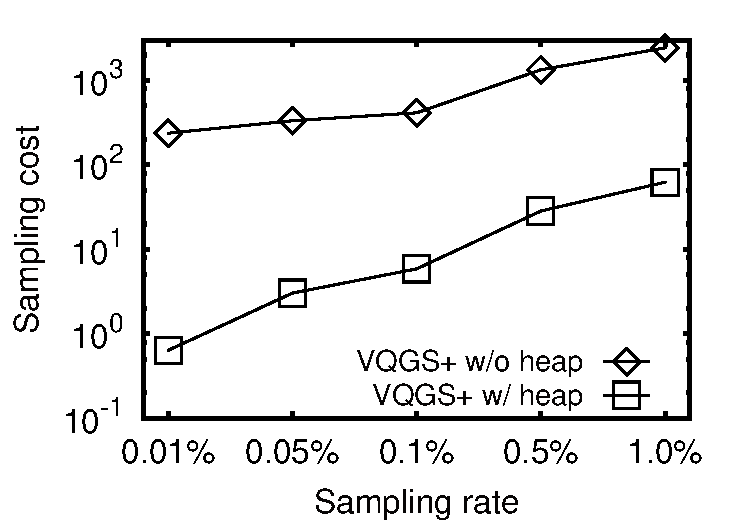
\includegraphics[width=0.3\linewidth]{pictures/quantitative_study/vqgs_porto_t}
		&
		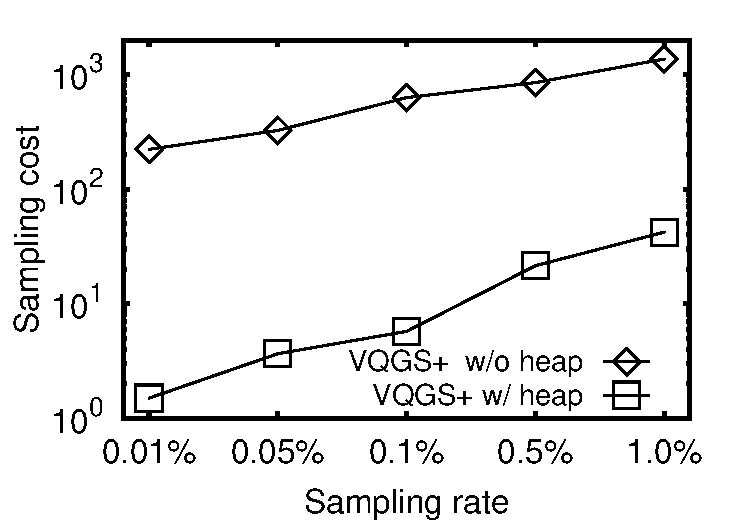
\includegraphics[width=0.3\linewidth]{pictures/quantitative_study/vqgs_sz_t}
		&
		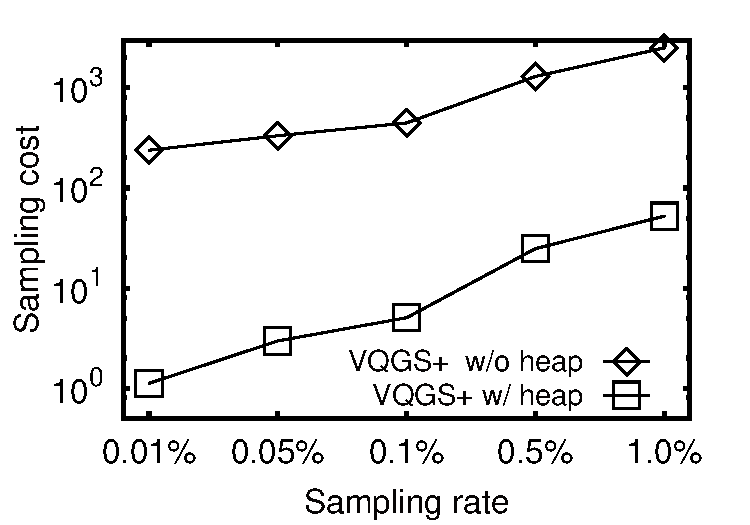
\includegraphics[width=0.3\linewidth]{pictures/quantitative_study/vqgs_cd_t}
		\\
		(A) \pt{}
		&
		(B) \sz{}
		&
		(C) \cd{}
	\end{tabular}
    \trim
	\caption{Effect of sampling rate on the sampling cost of $\vatss$ with/without optimization}
	\label{fig:rate_algtime}
	\trim \trim
\end{figure*}

\subsection{Quantitative Evaluation}\label{sec:quality}
In this part, we quantitatively evaluate the visual quality and efficiency of $\avats$ on the three real-world trajectory datasets.

\stitle{Visual quality} Figure~\ref{fig:rate_quality} reports the visualization quality (as defined in Equation~\eqref{eqref:loss}) of the methods under different sampling rate.
We consider the entire region in each dataset for this experiment.
The results show that our proposal $\avats$ achieves significantly higher quality than $\rand$ and $\mathsf{DTW}$ under the same sampling rate.
This is because the sampling algorithm $\vats$ and $\vatss$ in the $\avats$ framework are designed with explicit considerations for visual quality.
Specifically, the quality of $\avats$ approaches 1 when the sampling rate is still less than 1\% for all 3 datasets.
$\mathsf{DTW}$ has a higher quality than $\rand$ because it considers the diversity of trajectories.


In Figure~\ref{fig:rate_vistime}, we report the visualization cost (i.e., the wall clock time to generate visualization result using the sampled trajectories) for the methods under different sampling rate.
We still consider the entire region in this experiment and the visualization time of $\full$ (which does not change with sampling rate) is included at the top of each figure for reference.
The results show that all sampling methods achieve significantly shorter visualization cost than $\full$, and the speedup can be 1 to 4 orders of magnitude.
This confirms our observation that sampling is effective in improving visualization efficiency.
Under the same sampling rate, our $\avats$ takes slightly longer visualization time than $\rand$ and $\mathsf{DTW}$
because $\avats$ tends to select long trajectories for quality maximization.
%It is worth to point out the largest visualization cost of $\avats$ in \pt{}, \sz{} and \cd{} are 0.339, 0.275 and 0.471
Combining Figure~\ref{fig:rate_quality} and~\ref{fig:rate_vistime}, we can conclude that $\avats$ can achieve high visualization quality with  short visualization latency.


\stitle{Efficiency of $\avats$}
We evaluate the \textit{response time} of our $\avats$ framework under different quality guarantees and region sizes in Figure~\ref{fig:size_responsetime}.
The response time of $\avats$ is the end-to-end time for generating visualization for a selected region, which includes querying the $\avats$ index and computing the visualization.
For comparison, we also plot the response time of $\vatss$ (with $\delta\!=\!8$), which uses on-line sampling instead of querying the index in $\avats$ framework.
We constrain the regions to be rectangles with a constant height/width ratio and measure the size of a region by dividing its height over the height of the entire region.
For each region size, we report the average response time of three typical regions, i.e., a dense region, a sparse region and a medium region.
The results show that $\avats$ achieves a short response time (less than 1 second in all cases and 0.2 second for most cases) for different region sizes and quality guarantees. $\vatss$ is 1 to 2 orders of magnitude slower than $\avats$ and takes at most 14.802 seconds in all cases. These results show that $\vatss$ cannot support interactive visual exploration and the $\invQ$-tree index in $\avats$ is effective in improving efficiency.
In addition, the response time decreases rapidly when the region size shrinks as there are fewer trajectories in a smaller region.
However, the response time required to achieve a high quality (e.g., 0.9) is not significantly longer than a low quality (e.g., 0.7) as quality improves quickly with the number of sampled trajectories as a shown in Figure~\ref{fig:rate_quality}.





\stitle{Effect of heap-based lazy computation}
In Figure~\ref{fig:rate_algtime}, we report the running time of $\vatss$  with and without the heap-based lazy computation.
The results show that the heap-based optimization reduces the running time of $\vatss$ around 2 orders of magnitude.
For the sampling rates we considered, $\vatss$ runs efficiently and can finish within 1 second for the entire dataset.



%\begin{figure}[t]
%	\centering
%	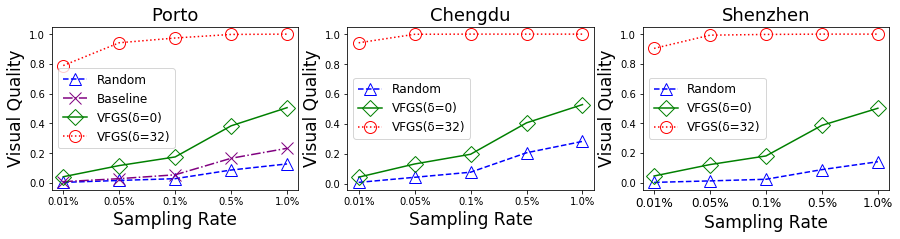
\includegraphics[width=0.5\textwidth]{pictures/quantitative_study_icde/sample_quality.png}
%	\vspace{-8mm}
%	\caption{Visual quality vs. sampling rates.}
%	\label{fig:sample_quality}
%	\vspace{-3mm}
%\end{figure}

%\begin{figure}[t]
%	\centering
%	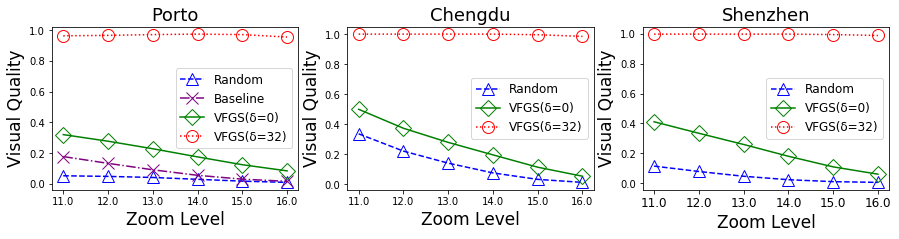
\includegraphics[width=0.5\textwidth]{pictures/quantitative_study_icde/zoom_quality.png}
%	\vspace{-8mm}
%	\caption{Visual quality vs. zoom level.}
%	\label{fig:zoom_quality}
%	\vspace{-3mm}
%\end{figure}


%\begin{table}
%	\centering
%	\small
%	\caption{The cost of $\invQ$-tree index}
%	\begin{tabular}{|@{}c@{}|@{}c@{}|@{}c@{}|@{}c@{}|@{}c@{}|} \hline
%		Dataset (size) & Height & Building time & Memory size \\ \hline
%		\pt{} (1.44G)	& 13 & 526.390s & 3.65GB  \\ \hline
%		\sz{} (1.02G)	& 13 & 435.291s  & 3.12GB \\ \hline
%		\cd{} (1.49G)	& 13 & 454.151s & 3.71GB \\ \hline
%	\end{tabular}	\label{tab:index cost}
%    \trim %\trim
%\end{table}

\begin{table}
	\centering
	\small
	\caption{The cost of $\invQ$-tree index}
	\begin{tabular}{|c|c|c|c|} \hline
		Dataset (size) & Height & Building time & Memory size \\ \hline
		\pt{} (1.44G)	& 13 & 526.390s & 3.65GB  \\ \hline
		\sz{} (1.02G)	& 13 & 435.291s  & 3.12GB \\ \hline
		\cd{} (1.49G)	& 13 & 454.151s & 3.71GB \\ \hline
	\end{tabular}	\label{tab:index cost}
	\trim %\trim
\end{table}

\stitle{$\invQ$-tree index cost evaluation}
We report the building time and memory cost of the $\invQ$-tree index in Table~\ref{tab:index cost}.
For all three datasets, it takes less than 10 minutes to build the $\invQ$ index with a height of 13.
The memory cost of the $\invQ$ index in the last column is also comparable with the size of the raw data shown in the first column.




%\stitle{Running time evaluation}

%\begin{figure}[t]
%	\centering
%	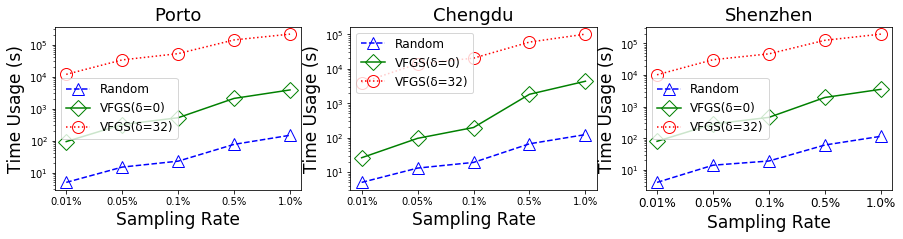
\includegraphics[width=0.5\textwidth]{pictures/quantitative_study_icde/sample_time.png}
%	\vspace{-8mm}
%	\caption{Time usage vs. sampling rates.}
%	\label{fig:sample_time}
%	\vspace{-3mm}
%\end{figure}

%\begin{figure}
%	\centering
%	\small
%	\begin{tabular}{cc}
%		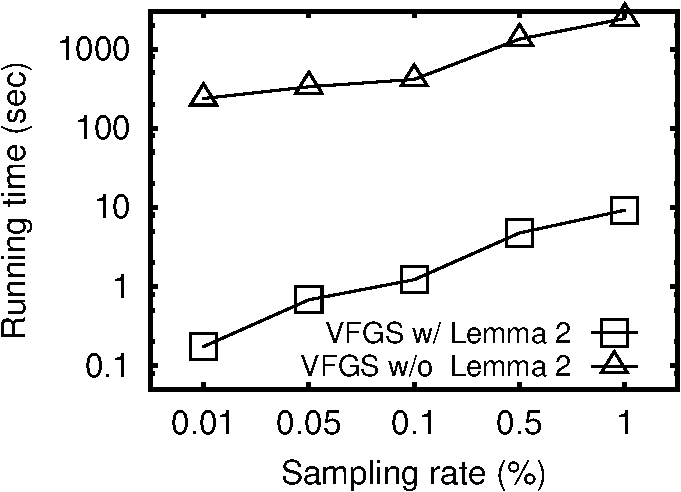
\includegraphics[width=0.44\columnwidth]{pictures/tporto}
%		&
%		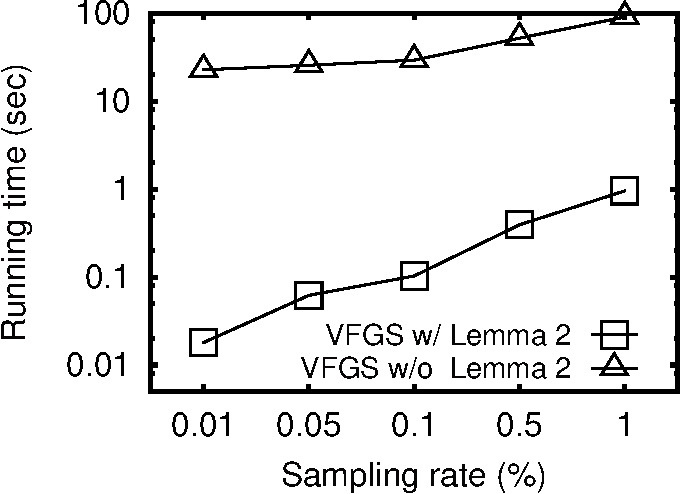
\includegraphics[width=0.44\columnwidth]{pictures/tshenzhen}
%		\\
%		(A) \pt{}
%		&
%		(B) \sz{}	
%	\end{tabular}
%	\vspace{-3mm}
%	\caption{Running time of $\vats$ w/ and w/o Lemma~\ref{lem:submodular}.}
%	\label{fig:cost}
%	\vspace{-6mm}
%\end{figure}
%\QM{unfininshed}
%We first conduct an experiment to evaluate the rendering cost by datasize. We vary the number of trajectories from 1000 to 1 million, which are randomly selected from \pt{} dataset. The experimental results are summarized in Table~\ref{tab:gpu}. We observe that the rendering cost is linear with the input data trajectories.
%
%We first report the running time of our $\vats$ algorithm in Figure~\ref{fig:cost} by varying the sampling rate from $0.01\%$ to $1\%$. The results show that $\vats$ is quite slow without the submodularity of contribution value, which agrees with Lemma~\ref{lem:submodular} in Section~\ref{sec:opt}.
%Then we shown the total time usage with sampling rate as Figure~\ref{fig:sample_time}. {*******}
%
%The optimized $\vats$ (e.g., $\vats$ with Lemma~\ref{lem:submodular}) outperforms $\vats$ by one to three orders of magnitudes on both datasets. The result show that running time of our $\vats$ algorithm is below 1 second in most cases. We have shown that $\vats$ provides good visualization performance with a low sampling rate (e.g., $0.1\%$ or $1\%$) in Section 6.1 and 6.2,  and Table~\ref{tab:gpu} suggests that the rendering latency scales almost linearly with dataset cardinality. By significantly reducing the dataset cardinality with sampling, $\vats$ can effectively reduces the rendering latency to make interactive visualization possible without sacrificing visual quality. For example, rendering the full $\pt{}$ dataset takes about \QM{34 seconds}, with a sampling rate of $1\%$, $\vats$ can bring down the rendering latency to less than 1 second.



